\documentclass[11pt,a4paper]{article}

% Packages
\usepackage[utf8]{inputenc}
\usepackage[T1]{fontenc}
\usepackage[french]{babel}
\usepackage{geometry}
\usepackage{graphicx}
\usepackage{float}
\usepackage{amsmath}
\usepackage{hyperref}
\usepackage{setspace}
\usepackage{caption}
\usepackage{subcaption}
\usepackage{enumitem}
\usepackage{listings}
\usepackage{xcolor}
\usepackage{pdfpages}
\usepackage{tikz}
\usetikzlibrary{shapes,arrows,positioning,fit,backgrounds}

\geometry{margin=2.5cm}
\onehalfspacing

% Configuration des listings
\lstset{
    basicstyle=\ttfamily\footnotesize,
    keywordstyle=\color{blue}\bfseries,
    commentstyle=\color{gray}\itshape,
    stringstyle=\color{red},
    showstringspaces=false,
    breaklines=true,
    frame=single,
    numbers=left,
    numberstyle=\tiny\color{gray},
    language=C++
}



\title{\textbf{Rapport de projet\\Application de gestion de tâches ToDoApp}}
\author{Simon Bélier \and Wissal Jalfa}
\date{\today}

\begin{document}

% Page de garde personnalisée
\begin{titlepage}
\centering

% Titre
{\huge\bfseries Rapport de projet\\[0.5cm]}
{\LARGE Application de gestion de tâches\\[0.3cm]}
{\LARGE\textbf{ToDoApp}}\\[1.5cm]

% Informations du cours
{\large\textbf{Cours : Langages et Applications Orientés Objets Avancés (LAOA)}}\\[1cm]

% Auteurs
{\large
\textbf{Auteurs :}\\[0.5cm]
Simon Bélier\\
Wissal Jalfa
}\\[1.5cm]

\vspace*{0.5cm}

% Logo ENSIIE en haut
\includegraphics[width=0.35\textwidth]{images/ensiie-logo.pdf}\\[1.5cm]

% Logos C++ et Qt6
% \vspace{1cm}
\begin{minipage}{0.4\textwidth}
\centering
\textbf{Technologies utilisées :}
\end{minipage}

% \vspace{0.5cm}
% Espace pour logos C++ et Qt6 (à ajouter si disponibles)
\includegraphics[height=3cm]{images/cpp-logo.jpg}
\hspace{1cm}
\includegraphics[height=3cm]{images/qt-logo.png}

\vfill

% Date
{\large \today}

\end{titlepage}

\tableofcontents
\newpage

% =================================================
\section{Introduction}
% =================================================

Ce rapport présente le projet ToDoApp, une application de gestion de tâches hiérarchiques développée en C++ avec le framework Qt 6.

\subsection{Contexte et évolution du projet}

À l'origine, le cahier des charges prévoyait une application simple de gestion de tâches permettant d'ajouter, modifier et supprimer des tâches avec quelques attributs basiques (titre, description, date d'échéance). Au fil du développement, le projet a considérablement évolué pour intégrer de nombreuses fonctionnalités avancées qui n'étaient pas initialement prévues :

\begin{itemize}
\item \textbf{Architecture hiérarchique} : Passage d'une liste plate de tâches à un système de tâches et sous-tâches de profondeur arbitraire avec \texttt{QAbstractItemModel}
\item \textbf{Intégration Git} : Ajout d'un système complet de synchronisation avec GitHub, GitLab et Gitea pour suivre les issues de projets externes
\item \textbf{Vues métier avancées} : Développement d'une vue Kanban, d'un widget de statistiques avec graphiques (distribution, heatmap, timeline, burndown chart)
\item \textbf{Fonctionnalités de productivité} : Timer Pomodoro, mode focus, calcul de séries (streaks), suivi de progression
\item \textbf{Système d'annulation} : Implémentation complète d'un système Undo/Redo avec \texttt{QUndoStack} et commandes personnalisées
\item \textbf{Export et persistance} : Support de multiples formats d'export (JSON, CSV, Markdown, PDF avec templates)
\item \textbf{Interface multilingue} : Système complet de traduction français/anglais avec détection automatique de la langue système
\item \textbf{Thèmes visuels} : Trois thèmes personnalisables (clair, sombre, chaleureux) avec feuilles de style QSS
\end{itemize}

Cette évolution progressive a transformé un projet simple en une application complète, tout en conservant une architecture MVC rigoureuse et une séparation claire des responsabilités.

\subsection{Architecture et technologies}

L'application implémente l'architecture MVC (Modèle-Vue-Contrôleur) et utilise les mécanismes de Qt pour synchroniser automatiquement les données et l'interface graphique.

Le projet démontre l'utilisation des concepts de Qt : modèles personnalisés dérivés de \texttt{QAbstractItemModel}, vues arborescentes (\texttt{QTreeView}), modèles proxy de filtrage (\texttt{QSortFilterProxyModel}), délégués d'édition (\texttt{QStyledItemDelegate}), et système de signaux/slots pour la communication inter-composants. L'application intègre des fonctionnalités avancées : système d'annulation/rétablissement (Undo/Redo) avec \texttt{QUndoStack}, intégration avec les plateformes Git (GitHub, GitLab, Gitea), vues métier (Kanban, Timeline, Burndown), et widgets de visualisation des statistiques.

L'architecture suit la séparation stricte des responsabilités : les classes de modèle (\texttt{Task}, \texttt{Category}, \texttt{TaskModel}) gèrent la logique métier et la persistance des données, les vues (\texttt{MainWindow}, \texttt{TaskDetailWidget}, \texttt{KanbanView}) gèrent l'affichage, et les contrôleurs coordonnent les interactions utilisateur.

% =================================================
\section{Architecture générale}
% =================================================

L'architecture de ToDoApp suit le patron MVC avec une séparation entre le modèle de données, les vues graphiques et la logique de contrôle. La figure \ref{fig:architecture} présente l'organisation des composants principaux et leurs interactions.

\begin{figure}[H]
\centering
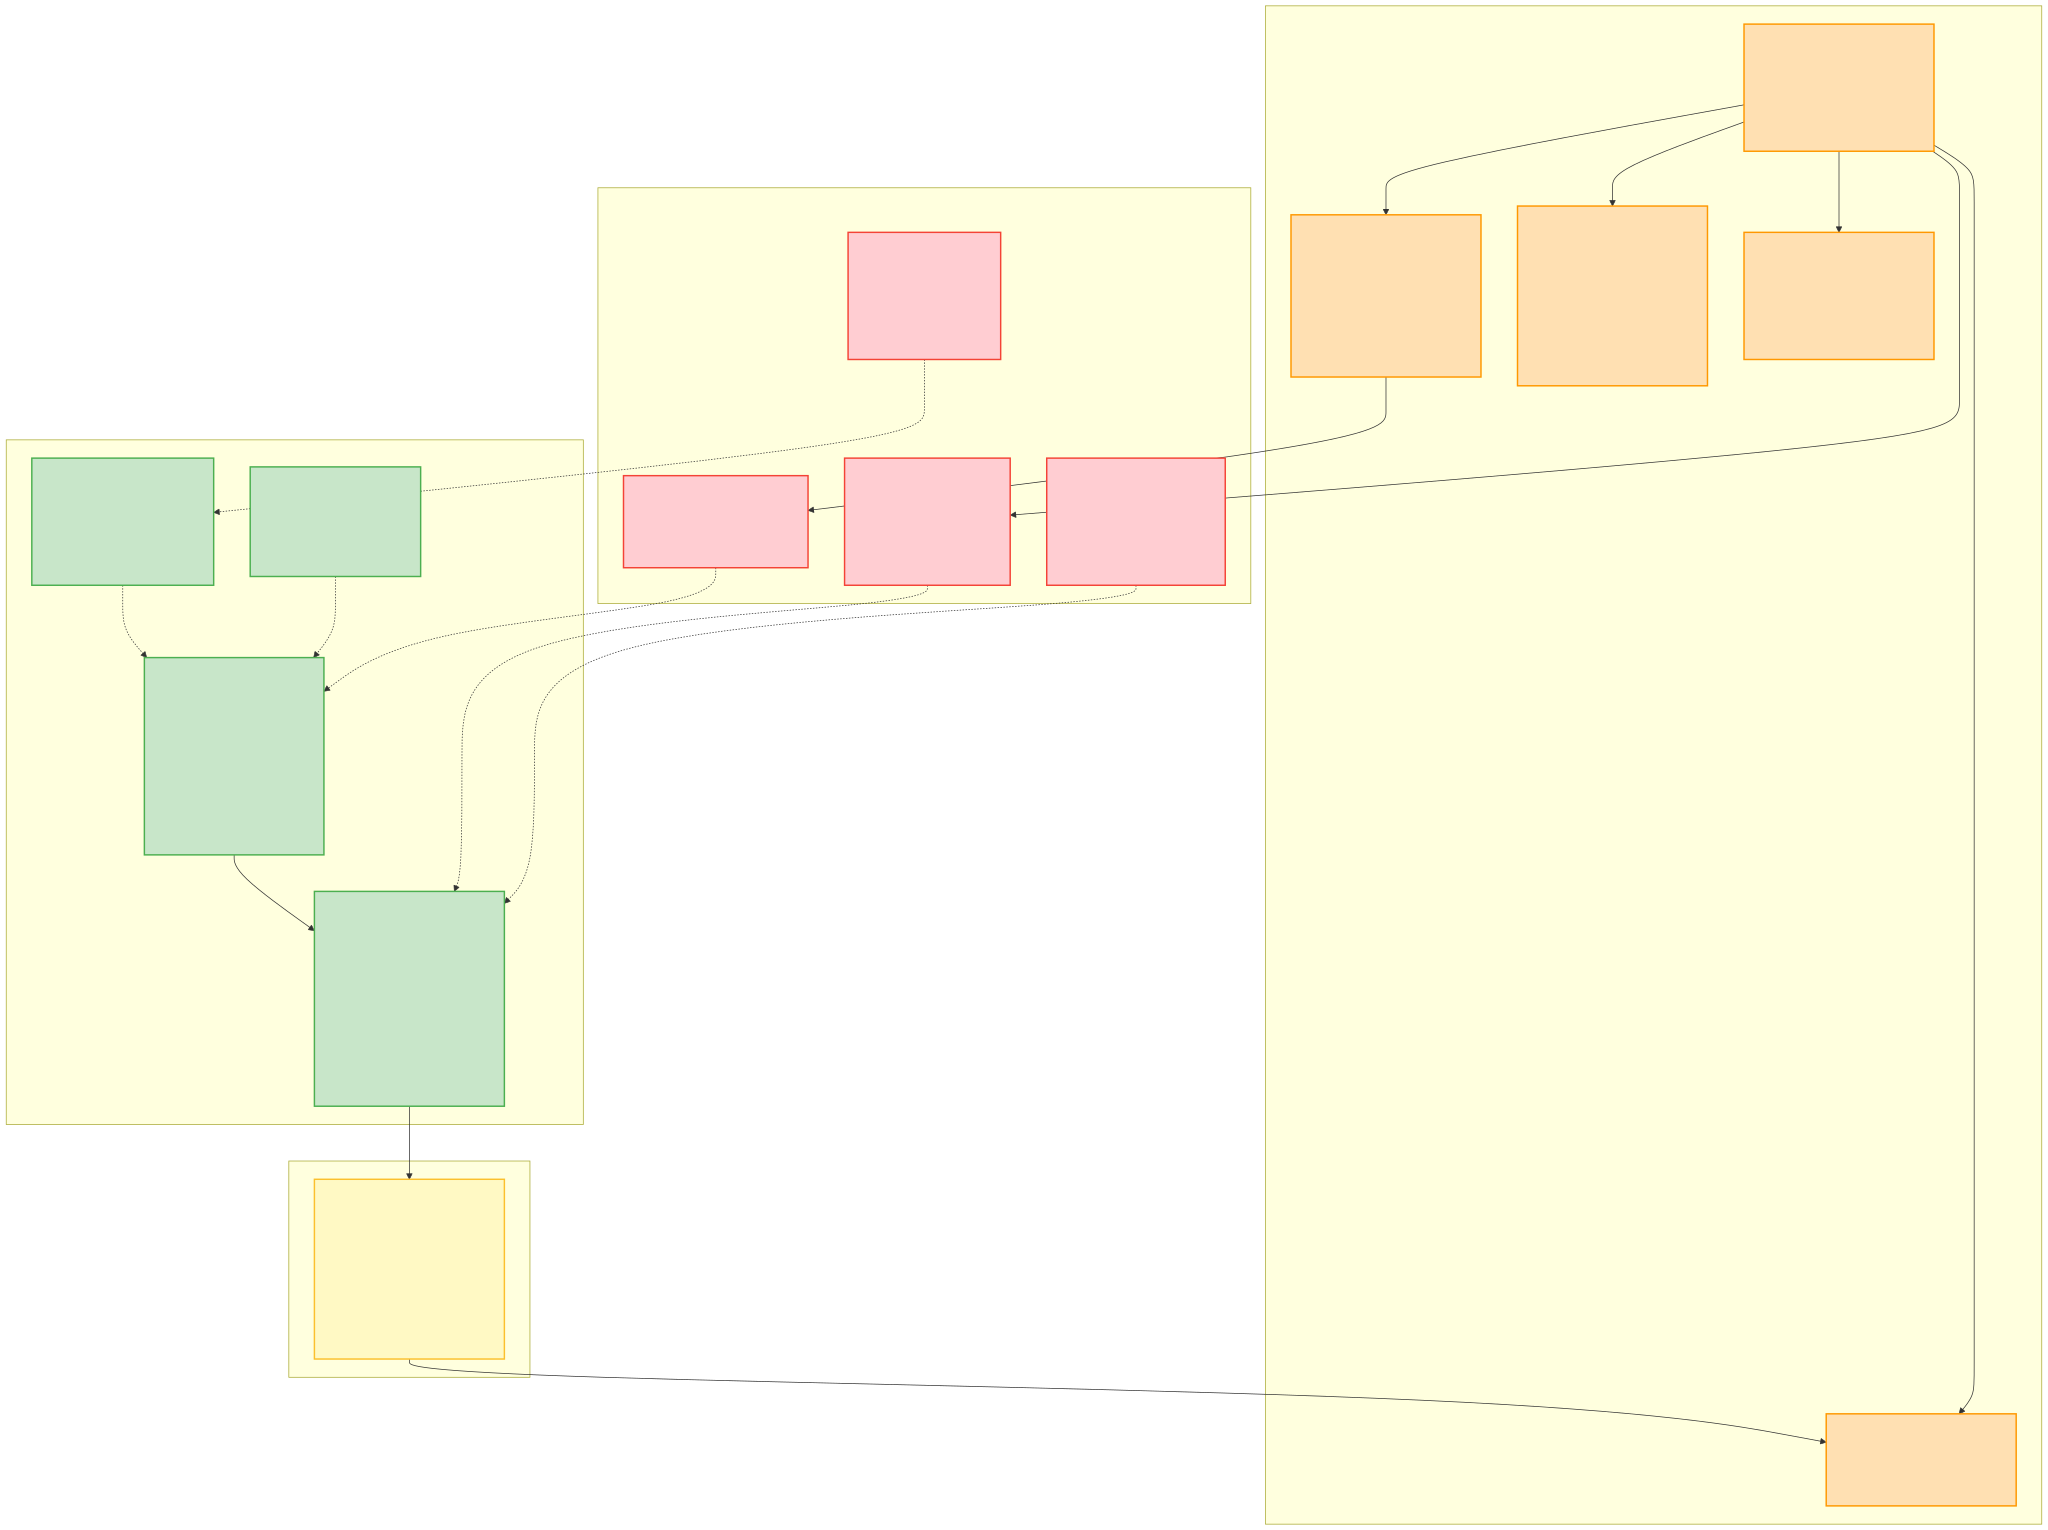
\includegraphics[angle=90,scale=1,keepaspectratio]{images/architecture_mvc.pdf}
\caption{Architecture MVC de l'application ToDoApp}
\label{fig:architecture}
\end{figure}


\begin{figure}[H]
\centering
\includegraphics[width=0.9\textwidth]{images/main_window_with_tasks.png}
\caption{Vue d'ensemble de l'interface principale avec tâches}
\label{fig:mainwindow-screenshot}
\end{figure}

Le modèle (\texttt{TaskModel}) hérite de \texttt{QAbstractItemModel} pour gérer la structure arborescente des tâches. Un proxy de filtrage (\texttt{TaskFilterProxyModel}) s'intercale entre le modèle et la vue (\texttt{QTreeView}) pour implémenter la recherche et le filtrage sans altérer les données sources. La fenêtre principale (\texttt{MainWindow}) orchestre les interactions et contient tous les widgets de visualisation.

% =================================================
\section{Classes et diagramme de classes}
% =================================================

\subsection{Inventaire des classes principales}

Le projet ToDoApp est structuré en quatre catégories de classes :

\paragraph{Classes du modèle métier} (répertoire \texttt{src/models/})
\begin{itemize}[noitemsep]
    \item \texttt{Task} : représentation d'une tâche avec hiérarchie parent-enfant
    \item \texttt{GitIssueTask} : extension de \texttt{Task} pour synchronisation Git
    \item \texttt{Category} : regroupement thématique de tâches
    \item \texttt{TaskModel} : modèle Qt arborescent (\texttt{QAbstractItemModel})
    \item \texttt{TaskFilterProxyModel} : proxy de filtrage et recherche
    \item \texttt{TaskItemDelegate} : délégué pour édition in-place
\end{itemize}

\paragraph{Classes de vue} (répertoire \texttt{src/widgets/})
\begin{itemize}[noitemsep]
    \item \texttt{MainWindow} : fenêtre principale et contrôleur central
    \item \texttt{TaskDetailWidget} : panneau d'édition exhaustive d'une tâche
    \item \texttt{KanbanView} : vue Kanban par colonnes de statut
    \item \texttt{StatisticsWidget} : affichage des métriques agrégées
    \item \texttt{ChartsWidget} : graphiques de répartition
    \item \texttt{TimelineWidget} : vue chronologique
    \item \texttt{BurndownWidget} : graphique de progression
    \item \texttt{HeatmapWidget} : carte de chaleur d'activité
    \item \texttt{PomodoroTimer} : timer Pomodoro
\end{itemize}

\paragraph{Classes utilitaires} (répertoire \texttt{src/utils/})
\begin{itemize}[noitemsep]
    \item \texttt{PersistenceManager} : sauvegarde/chargement JSON, CSV, Markdown
    \item \texttt{AddTaskCommand}, \texttt{RemoveTaskCommand}, \texttt{ModifyTaskCommand} : commandes Undo/Redo
    \item \texttt{ThemesManager} : gestion des thèmes visuels
\end{itemize}

\paragraph{Classes Git} (répertoire \texttt{src/git/})
\begin{itemize}[noitemsep]
    \item \texttt{RepositoryManager} : gestionnaire de dépôts Git
    \item \texttt{GitRepository} : représentation d'un dépôt distant
    \item \texttt{GitHubConnector}, \texttt{GitLabConnector} : connecteurs API REST
    \item \texttt{GitProjectWidget} : interface de gestion des dépôts
\end{itemize}

\subsection{Diagramme de classes détaillé}

La figure \ref{fig:classdiagram} présente le diagramme de classes complet mettant en évidence les relations d'héritage, de composition, et d'association entre les classes principales.

\begin{figure}[p]
\centering
\includegraphics[angle=90,scale=0.20,keepaspectratio]{images/diagramme_de_classe.pdf}
\caption{Diagramme de classes UML de ToDoApp}
\label{fig:classdiagram}
\end{figure}


\subsection{Relations entre les classes}

\paragraph{Héritage.} Toutes les classes métier (\texttt{Task}, \texttt{Category}) héritent de \texttt{QObject} pour bénéficier du système de signaux/slots. \texttt{GitIssueTask} étend \texttt{Task} pour ajouter les métadonnées Git. \texttt{TaskModel} hérite de \texttt{QAbstractItemModel} pour implémenter un modèle arborescent compatible avec les vues Qt.

\paragraph{Composition.} La classe \texttt{Task} implémente une relation de composition récursive : chaque tâche possède une liste de sous-tâches (\texttt{m\_subtasks}), permettant de construire des arbres de profondeur arbitraire. Le \texttt{TaskModel} possède également les tâches racines (\texttt{m\_rootTasks}) et est responsable de leur cycle de vie.

\paragraph{Agrégation.} La classe \texttt{Category} maintient une liste de références vers des tâches (\texttt{m\_tasks}) sans en avoir la propriété. La destruction d'une catégorie n'entraîne pas la destruction des tâches associées.

\paragraph{Association.} \texttt{TaskFilterProxyModel} observe \texttt{TaskModel} via les signaux Qt standard (\texttt{dataChanged}, \texttt{rowsInserted}). \texttt{MainWindow} orchestre l'ensemble des widgets et leur fournit une référence au modèle. Les widgets de visualisation (\texttt{KanbanView}, \texttt{ChartsWidget}) observent également le modèle pour se rafraîchir automatiquement.

% =================================================
\section{Modèle de données}
% =================================================

\subsection{La classe Task}

La classe \texttt{Task}, définie dans \texttt{task.h} et \texttt{task.cpp}, hérite de \texttt{QObject} et représente une tâche individuelle. Elle encapsule les attributs suivants :

\begin{lstlisting}
class Task : public QObject {
    Q_OBJECT
private:
    QUuid m_id;
    QString m_title;
    QString m_description;
    QDate m_dueDate;
    Priority m_priority;        // enum: LOW, MEDIUM, HIGH, CRITICAL
    Status m_status;            // enum: NOTSTARTED, INPROGRESS, COMPLETED, CANCELLED
    QStringList m_tags;
    QList<QUrl> m_attachments;
    int m_estimatedMinutes;
    int m_actualMinutes;
    QDate m_completionDate;
    QString m_linkedIssueId;    // format: "owner/repo#123"
    
    Task *m_parentTask;
    QList<Task*> m_subtasks;    // Composition
};
\end{lstlisting}

Chaque tâche possède un identifiant unique (\texttt{QUuid}) généré automatiquement à la construction. La hiérarchie parent-enfant est implémentée par composition : chaque tâche maintient un pointeur vers son parent (\texttt{m\_parentTask}) ainsi qu'une liste de pointeurs vers ses sous-tâches (\texttt{m\_subtasks}). Cette structure permet de représenter des arbres de profondeur arbitraire.

La classe \texttt{Task} expose l'ensemble de ses attributs via des propriétés Qt (\texttt{Q\_PROPERTY}), ce qui permet une liaison automatique avec les widgets de l'interface. Toute modification d'une propriété déclenche l'émission d'un signal dédié (\texttt{titleChanged()}, \texttt{priorityChanged()}, etc.), assurant ainsi la cohérence entre le modèle et les vues.

\subsection{Extension Git : GitIssueTask}

La classe \texttt{GitIssueTask}, définie dans \texttt{src/git/gitissuetask.h}, hérite de \texttt{Task} et ajoute les attributs nécessaires à la synchronisation avec les issues Git (GitHub, GitLab, Gitea) :

\begin{lstlisting}
class GitIssueTask : public Task {
private:
    int m_issueNumber;
    QString m_repositoryUrl;
    GitPlatform m_platform;     // enum: GitHub, GitLab, Gitea
    QStringList m_assignees;
    QString m_milestone;
    QDateTime m_lastSyncDate;
};
\end{lstlisting}

Cette extension permet de synchroniser bidirectionnellement les tâches locales avec les issues distantes. Les modifications apportées à une \texttt{GitIssueTask} peuvent être propagées vers la plateforme Git correspondante via les classes \texttt{GitHubConnector} et \texttt{GitLabConnector}.

\subsection{Le modèle Qt : TaskModel}

\subsubsection{Choix de QAbstractItemModel}

La classe \texttt{TaskModel}, définie dans \texttt{taskmodel.h} et \texttt{taskmodel.cpp}, hérite de \texttt{QAbstractItemModel}. Ce choix architectural est motivé par la nécessité de représenter une structure hiérarchique complexe tout en restant compatible avec les vues Qt standards (\texttt{QTreeView}, \texttt{QListView}). Contrairement à \texttt{QAbstractListModel} (modèle plat) ou \texttt{QAbstractTableModel} (modèle tabulaire), \texttt{QAbstractItemModel} permet de modéliser des arbres de profondeur arbitraire en implémentant la méthode \texttt{parent()} qui retourne l'index du parent d'un élément donné.

\subsubsection{Structure interne}

Le \texttt{TaskModel} maintient une liste des tâches racines (\texttt{m\_rootTasks}). Les sous-tâches sont accessibles récursivement via la méthode \texttt{Task::subtasks()}. Chaque \texttt{QModelIndex} retourné par le modèle utilise son pointeur interne (\texttt{internalPointer()}) pour référencer directement l'objet \texttt{Task} correspondant. Cette technique évite les recherches coûteuses lors de l'accès aux données.

\begin{lstlisting}
QModelIndex TaskModel::index(int row, int col, const QModelIndex &parent) const {
    Task *parentTask = parent.isValid() 
        ? static_cast<Task*>(parent.internalPointer()) 
        : nullptr;
    
    Task *child = parentTask 
        ? parentTask->subtasks().at(row)
        : m_rootTasks.at(row);
    
    return createIndex(row, col, child);
}
\end{lstlisting}

\subsubsection{Colonnes affichées}

Le modèle expose cinq colonnes (\texttt{columnCount() == 5}) correspondant aux propriétés essentielles d'une tâche : Titre, Date d'échéance, Priorité, Statut, et Étiquettes. La méthode \texttt{data()} retourne les valeurs appropriées selon le rôle Qt demandé (\texttt{Qt::DisplayRole}, \texttt{Qt::EditRole}, \texttt{Qt::BackgroundRole}, \texttt{Qt::ForegroundRole}). Les colonnes de priorité et de statut sont colorées dynamiquement selon le thème actif (clair ou sombre), et les dates d'échéance dépassées sont affichées en rouge.

\subsection{Filtrage : TaskFilterProxyModel}

La classe \texttt{TaskFilterProxyModel} hérite de \texttt{QSortFilterProxyModel} et s'intercale entre le \texttt{TaskModel} et la \texttt{QTreeView} pour filtrer dynamiquement les tâches affichées sans modifier les données sous-jacentes. Le proxy implémente la méthode \texttt{filterAcceptsRow()} qui détermine si une tâche doit être affichée selon plusieurs critères : recherche textuelle classique, recherche avancée avec préfixes (\texttt{tag:}, \texttt{priority:}, \texttt{status:}, \texttt{date:}), filtre par priorité, filtre par statut, et affichage/masquage des tâches terminées.

\subsection{Signaux et slots pour la synchronisation}

Le système de signaux et slots de Qt assure la communication asynchrone entre les composants. Les signaux définis dans \texttt{Task} notifient les changements d'état (\texttt{titleChanged()}, \texttt{priorityChanged()}, \texttt{statusChanged()}, \texttt{taskModified()}). Le \texttt{TaskModel} émet également des signaux personnalisés (\texttt{taskAdded()}, \texttt{taskRemoved()}, \texttt{taskUpdated()}). Ces signaux sont connectés dans \texttt{MainWindow::setupConnections()} pour déclencher la mise à jour de la barre d'état et des widgets statistiques.

% =================================================
\section{Vues graphiques et widgets}
% =================================================

\subsection{Organisation de l'interface}

L'interface graphique de ToDoApp est structurée selon le schéma présenté en figure \ref{fig:interface}. La fenêtre principale est divisée horizontalement par un \texttt{QSplitter}, séparant la vue arborescente (gauche) du panneau de visualisation (droite).

\begin{figure}[H]
\centering
\begin{tikzpicture}[node distance=0.3cm]
    % Conteneur principal
    \draw[thick] (0,0) rectangle (14,8);
    \node at (7,8.3) {\textbf{MainWindow (QMainWindow)}};
    
    % Toolbar
    \draw[fill=gray!20] (0.2,7.5) rectangle (13.8,7.8);
    \node at (1.5,7.65) [font=\tiny] {    Toolbar: Actions + Recherche + Filtres};
    
    % Splitter
    \draw[thick, dashed] (6,0.2) -- (6,7.3);
    
    % Partie gauche : TreeView
    \draw[fill=blue!10] (0.3,0.3) rectangle (5.8,7.2);
    \node at (3,6.8) {\textbf{QTreeView}};
    \node at (3,6.3) [font=\small] {Vue arborescente};
    \node at (3,5.9) [font=\small] {des tâches};
    \draw (0.5,5.5) rectangle (5.6,5.7);
    \node at (1.2,5.6) [font=\tiny] {Titre};
    \draw (0.5,5.2) rectangle (5.6,5.4);
    \node at (1.2,5.3) [font=\tiny] {-- Sous-tâche};
    \draw (0.5,4.9) rectangle (5.6,5.1);
    \node at (1.2,5.0) [font=\tiny] {Titre 2};
    
    % Partie droite : Panneau avec vues
    \draw[fill=green!10] (6.2,0.3) rectangle (13.7,7.2);
    
    % Barre verticale de sélection
    \draw[fill=orange!20] (6.3,0.4) rectangle (6.9,7.1);
    \node at (6.6,6.8) [font=\tiny, rotate=90] {Détails};
    \node at (6.6,6.0) [font=\tiny, rotate=90] {Stats};
    \node at (6.6,5.2) [font=\tiny, rotate=90] {Pomodoro};
    \node at (6.6,4.4) [font=\tiny, rotate=90] {Kanban};
    
    % Zone de contenu (QStackedWidget)
    \draw[fill=yellow!10] (7.1,0.4) rectangle (13.6,7.1);
    \node at (10.35,6.5) {\textbf{QStackedWidget}};
    \node at (10.35,6.0) [font=\small] {Vue active :};
    \node at (10.35,5.5) [font=\small] {TaskDetailWidget};
    
    % Exemple de contenu du DetailWidget
    \draw (7.3,4.8) rectangle (13.4,5.2);
    \node at (8.0,5.0) [font=\tiny] {Titre:};
    \draw (7.3,4.3) rectangle (13.4,4.7);
    \node at (8.5,4.5) [font=\tiny] {Description:};
    \draw (7.3,3.8) rectangle (9.5,4.2);
    \node at (8.2,4.0) [font=\tiny] {Priorité:};
    \draw (9.6,3.8) rectangle (11.8,4.2);
    \node at (10.5,4.0) [font=\tiny] {Statut:};
    
    % Statusbar
    \draw[fill=gray!20] (0.2,0) rectangle (13.8,0.2);
    \node at (2,0.1) [font=\tiny] {Total: 42 tâches | Complétées: 15 | En cours: 27};
    
\end{tikzpicture}
\caption{Organisation spatiale de l'interface graphique}
\label{fig:interface}
\end{figure}

\subsection{Fenêtre principale : MainWindow}

La classe \texttt{MainWindow} hérite de \texttt{QMainWindow} et orchestre l'ensemble de l'interface. Elle instancie le \texttt{TaskModel}, le \texttt{TaskFilterProxyModel}, et tous les widgets de visualisation. La toolbar principale contient des widgets intégrés : un \texttt{QLineEdit} pour la recherche, deux \texttt{QComboBox} pour les filtres de priorité et de statut.

\subsection{Vue arborescente (QTreeView)}

La \texttt{QTreeView} est configurée pour supporter l'édition in-place, la sélection multiple, et le glisser-déposer. Un délégué personnalisé \texttt{TaskItemDelegate} fournit des éditeurs contextuels selon la colonne : \texttt{QLineEdit} pour le titre, \texttt{QDateEdit} avec calendrier pour la date, \texttt{QComboBox} pour la priorité et le statut.

\subsection{Panneau de détails : TaskDetailWidget}

\texttt{TaskDetailWidget} est un widget pour l'édition complète d'une tâche sélectionnée. Il contient des champs pour le titre, la description (avec éditeur Markdown et 3 modes de visualisation), la date d'échéance, la priorité, le statut, les temps estimé et réel, les tags (avec autocomplétion), et les pièces jointes. Les modifications sont appliquées uniquement après un clic sur le bouton "Appliquer".

\begin{figure}[H]
\centering
\includegraphics[width=0.85\textwidth]{images/edit_widget.png}
\caption{Panneau de détails TaskDetailWidget (vue 1)}
\label{fig:taskdetail-screenshot}
\end{figure}

\begin{figure}[H]
\centering
\includegraphics[width=0.85\textwidth]{images/edit_widget2.png}
\caption{Panneau de détails TaskDetailWidget (vue 2)}
\label{fig:taskdetail-screenshot2}
\end{figure}

\subsection{Vue Kanban}

La classe \texttt{KanbanView} fournit une visualisation alternative avec quatre colonnes organisées par statut (À faire, En cours, Terminé, Annulé). Chaque colonne est un \texttt{QListWidget} qui supporte le glisser-déposer pour changer le statut d'une tâche. Le \texttt{KanbanView} observe le \texttt{TaskModel} et se met à jour automatiquement. Cette vue complète la vue arborescente : la vue arborescente affiche la décomposition hiérarchique des tâches, tandis que la vue Kanban les organise selon leur statut.

\begin{figure}[H]
\centering
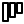
\includegraphics[width=0.9\textwidth]{images/kanban.png}
\caption{Vue Kanban avec colonnes par statut}
\label{fig:kanban-screenshot}
\end{figure}

% =================================================
\section{Contrôleurs et logique d'interaction}
% =================================================

\subsection{MainWindow comme contrôleur central}

La classe \texttt{MainWindow} agit comme le contrôleur central de l'application. La méthode \texttt{setupConnections()} établit l'ensemble des connexions signaux/slots : actions du menu aux slots correspondants, modèle de sélection de la \texttt{QTreeView} à \texttt{onTaskSelectionChanged()}, widgets de recherche au proxy model, \texttt{TaskDetailWidget} au modèle, et signaux du \texttt{TaskModel} à la barre d'état.

\subsection{Délégué d'édition : TaskItemDelegate}

\texttt{TaskItemDelegate} hérite de \texttt{QStyledItemDelegate} et personnalise l'édition in-place. Elle implémente \texttt{createEditor()} pour instancier le widget approprié, \texttt{setEditorData()} pour initialiser le widget avec la valeur actuelle, et \texttt{setModelData()} pour transmettre la nouvelle valeur au modèle via \texttt{setData()}.

\subsection{Système Undo/Redo}

L'application implémente un système complet basé sur \texttt{QUndoStack}. Trois commandes sont définies : \texttt{AddTaskCommand}, \texttt{RemoveTaskCommand}, et \texttt{ModifyTaskCommand}. Chaque commande hérite de \texttt{QUndoCommand} et implémente \texttt{undo()} et \texttt{redo()}. La pile d'annulation est accessible via Ctrl+Z et Ctrl+Shift+Z.

% =================================================
\section{Fonctionnalités de l'application}
% =================================================

\subsection{Création, modification, suppression}

L'utilisateur peut créer des tâches racines (Ctrl+N) ou des sous-tâches (Ctrl+Shift+N). L'édition se fait soit directement dans la \texttt{QTreeView} (double-clic), soit dans \texttt{TaskDetailWidget} (modifications appliquées via bouton "Appliquer"). La suppression (touche Suppr) est réversible via Undo/Redo, avec confirmation optionnelle.

\subsection{Filtrage et recherche}

Le \texttt{TaskFilterProxyModel} implémente plusieurs mécanismes : recherche textuelle classique, recherche avancée avec préfixes (\texttt{tag:urgent}, \texttt{priority:high}, \texttt{status:completed}, \texttt{date:2024-12}), filtres par priorité et statut via \texttt{QComboBox}, et affichage/masquage des tâches terminées.

\begin{figure}[H]
\centering
\includegraphics[width=0.9\textwidth]{images/filtrer1.png}\\
\vspace{0.3cm}
\includegraphics[width=0.9\textwidth]{images/filtrer2.png}\\
\vspace{0.3cm}
\includegraphics[width=0.9\textwidth]{images/filtrer3.png}
\caption{Interface de recherche et filtrage avancé (trois exemples)}
\label{fig:search-screenshot}
\end{figure}

\subsection{Statistiques et visualisations}

L'application intègre un \texttt{StatisticsWidget} qui affiche des métriques agrégées en temps réel : nombre total de tâches, taux de complétion, répartition par priorité et par statut, temps estimé vs temps réel, productivité quotidienne. Les widgets de visualisation incluent \texttt{ChartsWidget} (graphiques en camembert et barres), \texttt{TimelineWidget} (chronologie des tâches), \texttt{BurndownWidget} (courbe de progression), et \texttt{HeatmapWidget} (carte de chaleur d'activité hebdomadaire).

\subsubsection{Vue de distribution des tâches}

\begin{figure}[H]
\centering
\includegraphics[width=0.85\textwidth]{images/distribution.png}
\caption{Graphiques de distribution des tâches par priorité et statut}
\label{fig:distribution-screenshot}
\end{figure}

\subsubsection{Vue Heatmap}

La carte de chaleur (Heatmap) permet de visualiser l'activité hebdomadaire avec une représentation colorée de l'intensité de travail sur chaque jour.

\begin{figure}[H]
\centering
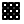
\includegraphics[width=0.8\textwidth]{images/heatmap.png}
\caption{Carte de chaleur d'activité hebdomadaire}
\label{fig:heatmap-screenshot}
\end{figure}

\begin{figure}[H]
\centering
\includegraphics[width=0.8\textwidth]{images/heatmap2.png}
\caption{Carte de chaleur d'activité (vue alternative)}
\label{fig:heatmap2-screenshot}
\end{figure}

\subsubsection{Vue Calendrier}

Le widget calendrier offre une vue chronologique des tâches avec leurs échéances.

\begin{figure}[H]
\centering
\includegraphics[width=0.85\textwidth]{images/calendrier.png}
\caption{Vue calendrier avec échéances des tâches}
\label{fig:calendrier-screenshot}
\end{figure}

\subsubsection{Vue d'avancement}

La vue d'avancement affiche la progression globale du projet sous forme de graphiques et métriques.

\begin{figure}[H]
\centering
\includegraphics[width=0.85\textwidth]{images/avancemnet.png}
\caption{Vue d'avancement du projet}
\label{fig:avancement-screenshot}
\end{figure}

\subsubsection{Timer Pomodoro}

L'application intègre un timer Pomodoro pour faciliter la gestion du temps de travail selon la technique Pomodoro.

\begin{figure}[H]
\centering
\includegraphics[width=0.6\textwidth]{images/pomodoro.png}
\caption{Timer Pomodoro intégré}
\label{fig:pomodoro-screenshot}
\end{figure}

\subsection{Persistance et export}

\texttt{PersistenceManager} fournit des méthodes statiques pour sauvegarder et charger des tâches en JSON (format natif préservant la hiérarchie), CSV (format tabulaire), Markdown (format texte avec niveaux de titres), et PDF (via template HTML et \texttt{QPrinter}). Un système de sauvegarde automatique périodique est paramétrable.

\subsection{Thèmes visuels}

L'application intègre un système complet de gestion des thèmes visuels via la classe \texttt{ThemesManager} (définie dans \texttt{src/utils/themesmanager.h}). L'utilisateur peut choisir parmi trois thèmes prédéfinis, chacun optimisé pour un contexte d'utilisation spécifique. Les thèmes sont implémentés via des feuilles de style Qt (QSS) stockées dans le répertoire \texttt{resources/themes/}.

\subsubsection{Thème clair (Light)}

Le thème clair fournit une interface lumineuse adaptée aux environnements bien éclairés. Il utilise des couleurs pastel et des contrastes modérés.

\begin{figure}[H]
\centering
\includegraphics[width=0.9\textwidth]{images/light_theme.png}
\caption{Interface avec thème clair}
\label{fig:light-theme-screenshot}
\end{figure}

\subsubsection{Thème sombre (Dark)}

Le thème sombre fournit une interface à dominante noire et grise, adaptée aux sessions de travail prolongées et aux environnements peu éclairés. Ce thème réduit la luminosité de l'écran tout en préservant la lisibilité.

\begin{figure}[H]
\centering
\includegraphics[width=0.9\textwidth]{images/dark_theme.png}
\caption{Interface avec thème sombre}
\label{fig:dark-theme-screenshot}
\end{figure}

\subsubsection{Thème chaleureux (Warm)}

Le thème chaleureux combine des tons chauds et une luminosité intermédiaire, servant de compromis entre les thèmes clair et sombre. Il utilise des nuances orangées et ambrées.

\begin{figure}[H]
\centering
\includegraphics[width=0.9\textwidth]{images/warm_theme.png}
\caption{Interface avec thème chaleureux}
\label{fig:warm-theme-screenshot}
\end{figure}

\paragraph{Implémentation technique.} Le \texttt{ThemesManager} charge dynamiquement les fichiers QSS correspondants et applique les feuilles de style via \texttt{QApplication::setStyleSheet()}. Le thème actif est sauvegardé dans les préférences utilisateur (\texttt{QSettings}) et restauré automatiquement au démarrage de l'application. Le changement de thème est instantané et n'affecte pas l'état des données ni des fenêtres ouvertes. Tous les widgets de l'application respectent automatiquement le thème actif grâce à l'utilisation systématique des classes de style Qt et à l'évitement des couleurs codées en dur dans le code C++.

\subsection{Intégration Git}

L'application propose un mode Git complémentaire (Ctrl+G) permettant de synchroniser les tâches avec les issues distantes (GitHub, GitLab, Gitea). \texttt{RepositoryManager} maintient une liste de dépôts configurés. \texttt{GitHubConnector} et \texttt{GitLabConnector} encapsulent les requêtes HTTP vers les API REST. \texttt{GitIssueTask} stocke les métadonnées Git supplémentaires (numéro d'issue, plateforme, assignés, milestone). La synchronisation bidirectionnelle permet de créer, mettre à jour, et importer des issues.

\begin{figure}[H]
\centering
\includegraphics[width=0.85\textwidth]{images/git_list_issues.png}
\caption{Liste des issues Git synchronisées}
\label{fig:git-list-screenshot}
\end{figure}

\begin{figure}[H]
\centering
\includegraphics[width=0.85\textwidth]{images/git_add_repo.png}
\caption{Interface d'ajout de dépôt Git}
\label{fig:git-add-screenshot}
\end{figure}

\paragraph{Architecture Git.} Le module Git s'articule autour de \texttt{GitProjectWidget} qui affiche la liste des dépôts configurés et permet d'ajouter/supprimer des connexions. Les connecteurs (\texttt{GitHubConnector}, \texttt{GitLabConnector}) héritent d'une interface commune et implémentent les appels API spécifiques à chaque plateforme. La synchronisation peut être manuelle (bouton "Sync") ou automatique (timer configurable). Les conflits de synchronisation sont détectés via les timestamps \texttt{lastSyncDate} et résolus selon une stratégie configurable (local prioritaire, distant prioritaire, ou demande utilisateur).

\subsection{Internationalisation et traductions}

L'application intègre un système complet d'internationalisation (i18n) via le framework de traduction Qt. Le projet prend en charge deux langues : le français (langue par défaut) et l'anglais américain. Les fichiers de traduction sont stockés dans le répertoire \texttt{translations/} :

\begin{itemize}
\item \texttt{ToDoApp\_fr.ts} : Fichier source de traduction française
\item \texttt{ToDoApp\_en\_US.ts} : Fichier source de traduction anglaise
\item \texttt{ToDoApp\_fr.qm} : Fichier compilé (binaire) pour le français
\item \texttt{ToDoApp\_en\_US.qm} : Fichier compilé (binaire) pour l'anglais
\end{itemize}

\paragraph{Gestion des traductions.} Les chaînes traduisibles dans le code C++ sont marquées avec la macro \texttt{tr()}, héritée de \texttt{QObject}. Pour les chaînes hors contexte de classe, la macro \texttt{QCoreApplication::translate()} est utilisée. Le système génère automatiquement les fichiers \texttt{.ts} via \texttt{lupdate}, qui extrait toutes les chaînes marquées comme traduisibles. Les traducteurs éditent ensuite ces fichiers XML via Qt Linguist, et \texttt{lrelease} les compile en fichiers \texttt{.qm} binaires chargés au runtime.

\paragraph{Détection de la langue.} Au démarrage, l'application détecte la langue du système via \texttt{QLocale::system().name()} et charge automatiquement le fichier de traduction correspondant. Si aucune traduction n'existe pour la langue système, l'application utilise le français par défaut. L'utilisateur peut changer la langue manuellement via le menu \texttt{Préférences > Langue}, et le changement prend effet immédiatement sans redémarrage grâce au mécanisme \texttt{QEvent::LanguageChange}.

\paragraph{Couverture des traductions.} L'ensemble de l'interface utilisateur est traduit : menus, boutons, labels, messages d'erreur, tooltips, et dialogues. Les traductions incluent également les formats de date et d'heure localisés via \texttt{QLocale::toString()}, ainsi que les pluriels gérés automatiquement par le système Qt (\texttt{\%n} dans les chaînes traduites). Le script \texttt{update\_translations.sh} automatise la mise à jour des fichiers de traduction lors de l'ajout de nouvelles chaînes dans le code.

% =================================================
\section{Justification des choix techniques}
% =================================================

\subsection{QAbstractItemModel pour la hiérarchie}

\texttt{QAbstractItemModel} est la seule classe Qt permettant de modéliser des arbres de profondeur arbitraire tout en restant compatible avec \texttt{QTreeView}. Un modèle plat ou tabulaire ne peut représenter la structure parent-enfant récursive des tâches et sous-tâches.

\subsection{Séparation MVC stricte}

La séparation MVC stricte garantit la testabilité (classes de modèle testables sans widgets), facilite l'évolution (ajout de nouvelles vues sans modifier le modèle), et permet la réutilisation (le \texttt{TaskModel} pourrait être utilisé dans un autre contexte). La synchronisation automatique via signaux Qt élimine les bugs liés à des états incohérents.

\subsection{Édition in-place}

L'édition in-place permet à l'utilisateur de modifier rapidement une valeur sans ouvrir de dialogue modal, ce qui est plus pratique. Cette approche suit les recommandations ergonomiques modernes (Material Design, Human Interface Guidelines).

\subsection{Proxy model pour le filtrage}

Le proxy préserve l'intégrité des données : le filtrage est purement présentationnel et n'affecte jamais le modèle source. Cette approche respecte le principe de responsabilité unique : \texttt{TaskModel} gère les données, \texttt{TaskFilterProxyModel} gère le filtrage.

\subsection{Intégration Git}

L'intégration Git permet aux équipes de développement qui utilisent GitHub/GitLab de synchroniser leurs issues. ToDoApp offre des vues complémentaires (Kanban, Timeline, Pomodoro) et des fonctionnalités absentes des interfaces web. La synchronisation bidirectionnelle évite la duplication des données.

% =================================================
\section{Conclusion}
% =================================================

Ce projet démontre une implémentation de l'architecture MVC avec Qt. L'application ToDoApp utilise les mécanismes du framework : modèles personnalisés dérivés de \texttt{QAbstractItemModel}, modèles proxy de filtrage, délégués d'édition, signaux et slots pour la synchronisation automatique, et framework Undo/Redo.

L'architecture est modulaire, testable et extensible. L'ajout de nouvelles fonctionnalités est possible sans modifier la structure existante grâce à la séparation des responsabilités et à l'utilisation des patterns de conception de Qt. Les fonctionnalités implémentées incluent les opérations de base (création, modification, suppression, filtrage, recherche, persistance) ainsi que des fonctionnalités avancées (intégration Git, vue Kanban, timer Pomodoro, visualisations statistiques).

\end{document}
